\chapter{Validations}
\label{sec:validations}

Once the scripts for \tool[] were completed I wanted to test how its usage could address the 2nd Challenge described in Chapter \ref{sec:background}, trying to automate the function-calls extraction and at the same time validate the accuracy of the tool as well the impact in the javascript ecosystem. In order to do that I performed 2 validation described as follows:

%Setup 
\section{Validation 1}

Since I had the result of the exploratory study performed previously I figured out that by replicating the study but using the tool to extract some of the information, I could get an estimation of the accuracy by comparing the results of both studies.
Since the data setup was already explained in Chapter \ref{sec:exploratory_study} please refer to that Chapter for details.
In this study I obtained the third party libraries function-calls, that were extracted manually on the previous study, by using the scripts of \tool[]. Based on the results from both studies I got the base values to make the calculations to obtain the accuracy of the tool among with other metrics. 

The base values are divided as follows:
\begin{itemize}
    \item \textbf{\textit{n}} represents the \textit{total number of projects} that where used in both studies.
    \item \textbf{\textit{TN}} represents the \textit{True Negative} results, this is obtained by cross-referencing the \textit{Actual No} values (i.e. those projects that where not using the vulnerable function in the exploratory study) and the \textit{Predicted No} values (i.e. those projects that where not using the vulnerable function according to \tool[]). 
    \item \textbf{\textit{FN}} represents the \textit{False Negatives} results, this is obtained by cross-referencing the \textit{Actual Yes} values (i.e. those projects that were using the vulnerable function in the exploratory study) and the \textit{Predicted No} values. 
    \item \textbf{\textit{FP}} represents the \textit{False Positives} results, this is obtained by cross-referencing the \textit{Actual No} values and the \textit{Predicted Yes} values (i.e. those projects that where using the vulnerable function according to \tool[]).
    \item \textbf{\textit{TP}} represents the \textit{True Positives} results, this is obtained by cross-referencing the \textit{Actual Yes} values and the \textit{Predicted Yes} values.
\end{itemize}
Figure \ref{fig:replicationStatistics} presents a template of how the base values were obtained.

%%%%%%%%%%%%%%%%%%%%%%%%%%%%%%%%%%%%%
\begin{figure}[ht]
\centering
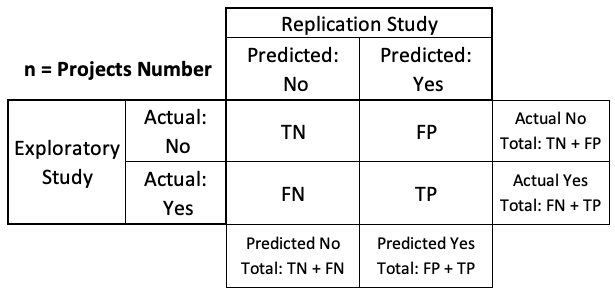
\includegraphics[width=1\textwidth]{images/replication_statistics.png}
\caption{Template for base values acquisition}
\label{fig:replicationStatistics}
\end{figure}
%%%%%%%%%%%%%%%%%%%%%%%%%%%%%%%%%%%%%

Once the base values where acquired the following metrics where calculated:
\begin{itemize}
    \item \textbf{\textit{Accuracy}} represents the percentage of the function-calls in a project that were identified accurately. This is obtained by adding the results of the \textit{True Negative} and \textit{True Positive} values and dividing them among the \textit{total number of projects}.
    \item \textbf{\textit{Miss-classification rate}} represents the percentage of the function-calls in a project that were identified inaccurately. This is obtained by adding the results of the \textit{False Positive} and \textit{False Negative} values and diving them among the \textit{total number of projects}.
    \item \textbf{\textit{TP rate}} represent the percentage of \textit{True Positive} values accurately detected. This is obtained by dividing the \textit{True Positive} result among the addition of \textit{False Negative} and \textit{True Positive} values.
    \item \textbf{\textit{FP rate}} represent the percentage of \textit{True Negative} values inaccurately detected. This is obtained by dividing the \textit{False Positive} values among the addition of \textit{True Negative} and \textit{False Positive} values.
    \item \textbf{\textit{TN rate}} represent the percentage of \textit{True Negative} values accurately detected. This is obtained by dividing the \textit{True Negative} values among the addition of \textit{True Negative} and \textit{False Positive} values.
    \item \textbf{\textit{FN rate}} represent the percentage of \textit{True Positive} values inaccurately detected. This is obtained by dividing the \textit{False Negative} values among the addition of \textit{False Negative} and \textit{True Positive} values.
\end{itemize}

\section{Validation 2}
For the previous studies I have hand-picked the projects, reason why for this study, first I wanted to perform an analysis on a larger scale sample to generalize my previous findings and second, I wanted to use a sample from the wild (i.e. a sample that was not carefully selected).  


I decided to run the analysis on a percentage of the sample used on the study performed by Decan et al. \cite{decan2018impact} and I used a similar approach of that used in the exploratory study previously described in this thesis and it will be detailed in three steps.
\begin{itemize}
    \item \textbf{Step One: Extract the Vulnerable Dependencies and Identify their Vulnerable Function}\\
    From the study performed by Decan et al. \cite{decan2018impact} I extracted a percentage of the vulnerabilities used and then using the information provided on the Snyk website\footnote{data was mined from website \url{https://snyk.io/vuln}} identified the vulnerable function of the vulnerable third-party library.
    
    \item \textbf{Step Two: Identify and Collect Client Projects} \\
    Taking the output from Step One, for Step Two I mined and collected npmJS projects\footnote{data was mined from the npmjs website at \url{https://www.npmjs.com}} from GitHub that used the vulnerable dependency. Then analyzing the last version available of the project I identified whether or not the client was using the vulnerable function.
    
    \item \textbf{Step Three: Usage Analysis}
    Taking the output for Step One and Two, for Step Three, using \tool[] I classified the output for the client projects as follows: (i) Dependency listed but not used (i.e. the third-party library was included in the dependencies but no function-calls were identified), (ii) Dependency is used (i.e the third-party library was included in the dependencies and function-calls were identified) and (iii) Unavailable (i.e. \tool[] could not retrieve information from the GitHub project repository). For the usage analysis I will be focusing on the \textit{Dependency is used} section and therefor the output will be divided in two patterns:
    \begin{enumerate}
        \item \textit{Used}: refers to clients that are using the vulnerable function of the vulnerable third-party library.
        \item \textit{Clean}: refers to clients that are not using the vulnerable function of the vulnerable third-party library.
    \end{enumerate}
\end{itemize}

In the analysis results I will be reporting the proportion of projects using the vulnerable function and those that are not using it. My intention is to determine how accurate is the assumption that a project is vulnerable only because it is using a vulnerable library.

%\section{Impact Study Setup}
For the selection of the vulnerable dependencies I randomly selected a 5\% of the vulnerabilities used in the study performed by Decan et al. \cite{decan2018impact} resulting in an set of 20 vulnerabilities. 
Once the vulnerabilities were selected, using the information provided by Snyk website, I manually traced the vulnerable function of the third-party library. Table \ref{tab:impactVulnerabilities} presents a summary of the vulnerable dependencies selected.

%%%%%%%%%%%%%%%%%%%%%%%%%%%%%%%%%%
\begin{table*}[ht]
\centering
\hspace*{-2cm}
\scalebox{0.7}{
\begin{tabular}{|l|l|l|l|l|}
\hline
\multicolumn{1}{|c|}{\textbf{Dependency}} & \multicolumn{1}{c|}{\textbf{Severity}} & \multicolumn{1}{c|}{\textbf{Snyk ID}} & \multicolumn{1}{c|}{\textbf{Published in Snyk}} & \multicolumn{1}{c|}{\textbf{Vulnerable Functions}} \\ \hline
angular & High & npm:angular:20150807 & 23 Jan 2017 & CompileProvider, module \\ \hline
bittorrent-dht & Medium & npm:bittorrent-dht:20160104 & 5 Jan 2016 & addNode, main\_method \\ \hline
boom & Medium & npm:boom:20130209 & 5 Oct 2016 & badRequest, unauthorized, clientTimeout, forbidden \\ \hline
bootstrap & Medium & npm:bootstrap:20120510 & 10 Apr 2017 & setContent \\ \hline
generator-jhipster & Medium & npm:generator-jhipster:20151006 & 28 Mar 2017 & validateToken \\ \hline
hapi & Low & npm:hapi:20151020 & 6 Nov 2015 & Server \\ \hline
hoek & Medium & npm:hoek:20130326 & 10 Nov 2016 & callStack, escapeHeaderAttribute, printEvent \\ \hline
minimatch & High & npm:minimatch:20160620 & 20 Jun 2016 & parse, main\_method \\ \hline
mongoose & High & npm:mongoose:20150925 & 13 Dec 2016 & validate \\ \hline
npm & Medium & npm:npm:20130708 & 13 Feb 2017 & setUser, cache \\ \hline
qs & High & npm:qs:20140806 & 6 Aug 2014 & compact, parseObject, parseString \\ \hline
react & High & npm:react:20150318 & 18 Jan 2017 & createClass \\ \hline
riot & Medium & npm:riot:20131114 & 8 May 2017 & render \\ \hline
sails & High & npm:sails:20161013 & 20 Oct 2016 & main\_method, initialize \\ \hline
sails & High & npm:sails:20130622 & 30 Jan 2017 & route, interpret \\ \hline
sequelize & Medium & npm:sequelize:20150517 & 1 Apr 2016 & no info found \\ \hline
socket.io & Medium & npm:socket.io:20120417 & 13 Feb 2017 & defaultTransports, handleHandshake \\ \hline
st & Medium & npm:st:20140206 & 6 Feb 2014 & st, main\_method \\ \hline
validator & Medium & npm:validator:20130705-2 & 5 Jul 2013 & xss\_clean \\ \hline
ws & High & npm:ws:20160624 & 26 Jun 2016 & WebSocketServer, Server \\ \hline
\end{tabular}}
\caption{Summary of the twenty Selected Vulnerable Dependencies}
\label{tab:impactVulnerabilities}
\end{table*}
%%%%%%%%%%%%%%%%%%%%%%%%%%%%%%%%%%

For the client selection I randomly selected 10 projects that were using the vulnerable library resulting in 200 client projects for the case study. 

Once the client projects were selected I downloaded the related GitHub repositories and analyzed the latest version available for every project with \tool[]. With the output generated by the tool I manually validated if the vulnerable functions were been called or not.